
\section{Introduction}

%Array programming is the core abstraction behind many of the modern miracles of computing (e.g. neural networks, scientific simulation, database processing). 
Arrays are the most fundamental abstraction in computer science. Arrays and lists are often the first-taught datastructure
\cite[Chapter 2.2]{abelson_structure_1996}, \cite[Chapter 2.2]{knuth_art_1997}.
%
Arrays are also universal across programming languages, from their introduction
in Fortran in 1957 to present-day languages like Python
\cite{backus_fortran_1957}, keeping more-or-less the same semantics.
%
Modern
array programming languages such as NumPy, SciPy, MatLab, TensorFlow, PyTorch,
and Halide have pushed the limits of productive data processing with arrays,
fueling breakthroughs in machine learning, scientific computing, image
processing, and more  \cite{harris_array_2020, virtanen_scipy_2020,
moler_history_2020, abadi_tensorflow_2016,
paszke_pytorch_2019,ragan-kelley_halide_2013}.
%
These frameworks have been the
subject of extensive industry investment to enable performant implementations,
and often operate at the peak capacity of the hardware they run on
\cite{lo_roofline_2015}.

The success and ubiquity of arrays is likely due to their simplicity. 
%
Since
their introduction, multidimensional arrays have represented dense, rectilinear,
integer grids of points. 
%
By \textbf{dense}, we mean that indices are mapped to value via a simple formula relating multidimensional space to linear memory.
%
\teo{Since the gap between the array storage and the array representation is minimal, dense arrays offer extensive compiler optimizations and extensive convenience.
%
Compilers understand dense array computation over
}
%
This
simplicity enables extensive interoperability, convenience layers, and
optimizations by breaking the abstraction barrier between array representation
and array storage.  
%
Compilers understand dense array computations across many
programming constructs, such as for and while loops, breaks, parallelism,
caching, prefetching, multiple outputs, scatters, gathers, vectoriation,
loop-carry-dependencies, and more. Several optimizations have been developed for
dense arrays, such as loop fusion, loop tiling, loop unrolling, and loop
interchange.
%
However, while dense arrays are the easiest way to program, the world is not all dense.

%Bring in structure
% - old arrays are Dense, rectilinear, integer grids
% - The world is not like that
% - Sparsity, runs of repeated values, symmetry
% - Lots of citations, perhaps a few figures from my powerpoint
%Sparse arrays
% - Networks (graphblas, graph frameworks)
% - Simulations (BLAS, symblas, banded blas, etc)
% - Databases (database engines)
%Run-length encoding
%Symmetry
%Bands
%Padding
%Blocks

\begin{figure}
	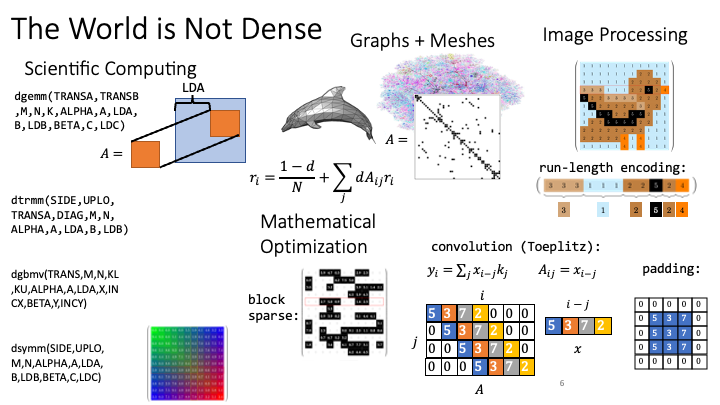
\includegraphics[width=\linewidth]{example_structures.png}
    \caption{some example structures that might be nice to put into a figure}
\end{figure}
Our world is full of structured arrays.
%
Sparse arrays (which store only nonzero elements) describe networks, databases, and simulations~\cite{abhyankarpetsc, bell2007lessons, mcauley2013hidden, balay2020petsc}.
%
Run-length encoding describes images and masks, geometry, and
databases (such as a list of transactions with the date field all the same)~\cite{shi2020column,golomb1966run}.
%
Symmetry, bands, padding, and blocks arise due to modeling choices in scientific computing (e.g. higher order FEMs) as well as in intermediate structures in many linear solvers (e.g. GMRES)~\cite{ded, saad2003iterative, o2009scientific}.
%
In the context of machine learning, combinations of sparse and blocked matrices are increasingly under consideration~\cite{dao2022monarch}.
%
Operators, such as convolution, can be expressed as structured arrays.
%
For example, a convolution with a filter can be expressed as a matrix multiplication
with the toeplitz matrix of all the circular shifts of the filter~\cite{sze2017efficient}.


%
\textbf{Currently, support for structured data is fragmented and incomplete}.
%
Experts must hand write variations of even the simplest kernels, like matrix
multiply, for each data structure/data set and architecture to get performance.
%
Implementations must choose a small set of features to support well, resulting
in a compromise between \textbf{program flexibility} and \textbf{data structure
flexibility}.
%
Hand-written solutions are collected in diverse libraries like
MKL, OpenCV, LAPACK or SciPy~\cite{ bradski2000opencv, anderson1999lapack, virtanen2020scipy, psarras2022linear}. 
%
However, libraries will only ever support a subset of
programs on a subset of data structure combinations.
%
Even the most advanced
libraries, such as the GraphBLAS, which support a wide variety of sparse
operations over various semi-rings always lack support for other features, such
as tensors, fused outputs, or runs of repeated values~\cite{bulucc2017design, mattson2019lagraph}.
%
While dense array
compilers support an enormous variety of program constructs like early break and
multiple left hand sides, they only support dense arrays~\cite{ragan-kelley_halide_2013,grosser2012polly}.  
%
Special-purpose
compilers like TACO, Taichi, StructTensor, or CoRa which support a select subset of structured data
structures (only sparse, or only ragged arrays) must compromise by greatly
constraining the classes of programs which they support, such as tensor
contractions \cite{kjolstad_tensor_2019, hu_taichi_2019, ghorbani2023compiling, fegade_cora_2022}. 
%
This trade-off is visualized in Tables \ref{tab:features} and \ref{tab:data_structures}.
%


\begin{table}[h!]
  \help{This table needs citations, as well as a little bit of double checking}
  \centering
  \begin{tabular}{l|cccccc}
  \textbf{Feature / Tool} & \textbf{Halide} & \textbf{Taco} & \textbf{Cora} & \textbf{Taichi} & \textbf{StructTensor} & \textbf{Finch} \\
  \hline
  Einsums and Contractions & \checkmark & \checkmark & \checkmark & \checkmark & \checkmark & \checkmark \\
  High-Level API           &            & \checkmark &            &            &            & \checkmark \\
  Automatic API Fusion     &            &            &            &            &            & \checkmark \\
%  Parallelism             & \checkmark & \checkmark & \checkmark & \checkmark&           & \checkmark \\
  Multiple LHS             & \checkmark &            & \checkmark & \checkmark &            & \checkmark \\
  Affine Indices           & \checkmark &            &            & \checkmark & \checkmark & \checkmark \\
  Recurrence               & \checkmark &            &            &            &            &           \\
  If-Conditions and Masks  & \checkmark & \checkmark &            & \checkmark &            & \checkmark \\
  Scatter Gather           & \checkmark &            &            & \checkmark &            &\checkmark \\
  Early Break              &            & \checkmark &            & \checkmark &            &\checkmark \\
  \end{tabular}
  \caption{Feature support across various tools.}
  \label{tab:features}
  \end{table}
  
  \begin{table}[h!]
  \centering
  \begin{tabular}{l|cccccc}
  \textbf{Feature / Tool} & \textbf{Halide} & \textbf{Taco} & \textbf{Cora} & \textbf{Taichi} & \textbf{StructTensor} & \textbf{Finch} \\
  \hline
  Dense                    & \checkmark & \checkmark & \checkmark & \checkmark & \checkmark & \checkmark \\
  Padded                   & \checkmark &            &            &            &            & \checkmark \\
  One Sparse               &            & \checkmark &            & \checkmark &            &\checkmark \\
  Sparse                   &            & \checkmark &            &            &            &\checkmark \\
  Run-length               &            &            &            &            &            & \checkmark \\
  Symmetric                &            &            &            &            & \checkmark & \checkmark \\
  Regular Sparse Blocks    &            & \checkmark &            &            &            & \checkmark \\
  Irregular Sparse Blocks  &            &            &            &            &            &\checkmark \\
  Ragged                   &            &            & \checkmark &            &            & \checkmark \\
  \end{tabular}
  \caption{Support for various data structures across tools. Finch supports \textbf{both} complex programs and complex data structures.}
  \label{tab:data_structures}
\end{table}

\teo{ New paragraph:
%
Many of these special purpose compilers represent a program's control flow via a specialized representation that is tightly integrated with a narrow class of supported data structures.
%
For example, TACO's merge lattices represent iterations over subsets of rectangular integer grids where computations produce non-zero values whereas the polyhedral model allows various compilers to represent dense computations on irregular regions~\cite{kjolstad_tensor_2017, grosser2012polly}.
%
Taichi enriches single static assignment form with specialized instruction for accessing a single sparse structure drawn from a particular class, which is why it supports the most control flow for a single sparse structure~\cite{hu_taichi_2019}.
%
Furthermore, the limits and advantages of a DSL can be traced to the specific coupling of a program's control flow with the data structure: many new TACO features required modifying algorithms that worked with TACO's merge lattices and Tiramisu can express programs that Halide can't because Tiramisu uses a polyhedral model as opposed to a model built on iterating over regular grids~\cite{kjolstad_tensor_2017, henry_compilation_2021, senanayake2020sparse, baghdadi2019tiramisu}.
%
In this work, we will choose  a new representation of a program's data structures and control flows that covers a wide range of programs.
%
However, simply combining a large variety of structured data with a large variety of programs does not necessarily yield a performance advantages.
%
To find and produce efficient programs for structured data, we must overcome two challenges that occur when we intersect complex control flow with structured data:}

%before introducing this, we must discuss performance: if we want to also produce efficient code for structured data, we face two challenges.



%build on some conception of an iteration space: TACO has merge lattices, Polyhedral compilers rely on the polyhedral model, Halide and Corra uses rectangular intervals, and so on.
%
%And we believe the limitations of these systems can be traced back to their specific conceptions.} \willow{I agree with what this sentence is saying, but I'm concerned that the sentiment is unclear, because here it may seem like we say "iteration space bad" and later say "iteration space good". Can we perhaps adjust here to say may of these special purpose compilers use overly restrictive models of the iteration space of the program, but that Finch is good because it uses general control flow to express a wider variety of iteration spaces. At a high level, we need to define "iteration space" or "control flow" or "Looplets" if we want to use them in the intro, and depending on how much we want to use these words we may want to avoid them here.}
%
% \teo{For example, each modification to expressions that TACO could support required modifying the merge lattice algorithms\cite{kjolstad_tensor_2017, henry_compilation_2021, senanayake2020sparse} and several programs could not be supported in Halide, but could be in Tiramisu due to the limitations of a rectangular iteration space~\cite{baghdadi2019tiramisu}.
% %
% And many iteration space concepts simply don't allow for skipping work that isn't simply the complement of an interval.
% %
% In our work, we will show how we can use Looplets as our main tool to manage the iteration spaces of our computations and data structures.
% %
% However, to support as many data structures and iteration spaces as is implied above, we face two challenges if we want to also produce efficient code over structured data.
% }
%We see two main challenges to writing efficient code over structured data.

\textbf{Optimizations are specific to the indirection and patterns in data structures}: 
%
These structures break the simple mapping between array elements and where they are stored in memory.
%
For example, sparse arrays store lists of which coordinates are nonzero, whereas run-length-encoded arrays map several pixels to the same color value. 
%
These zero regions or repeated regions are optimization opportunities, and we must adapt the program to avoid repetitive work on these regions by referencing the stored structure.

\textbf{Performance is highly structure dependent}: Structure aware kernels are dramatically faster than unstructured ones, and the landscape of implementation decisions is dramatically unpredictable. 
%
For example, sparse kernels don't need to compute on zeros, but this means that the precise input nonzero patterns act as computational filters, affecting the runtime as they interact with each other and the implementation.


\teo{We could add a third here: making intersections worth it.}
%\teo{Data structure driven array program performance engineering?}

%% Modification: We don't propose to fix these directly, but we do propose a programming model where they can be dealt with 
%% By supporting the features above, 


\teo{Proposed new paragraph:}

\teo{We don't propose to solve these problems automatically, but we do propose a new programming language where these issues are solvable, by virtue of the precise manner in which we combine structured data and control flow.}
%
\teo{Our language, Finch, combines structured data and control flow in a predictable manner by lowering both of them into an abstraction: Looplets~\cite{ahrens_looplets_2023}, which combines structured iterators into a single control flow that only produces the relevant portions of the output.}
%
\teo{For example, if a programmer wanted to merge the even indices of two sorted arrays, a programmer could represent by point-wise multiplying two sparse vectors to produce another sparse vector and then set the even indices two zero or the programmer could only point-wise multiply the two sparse vectors under an if condition that selects even indices. (This crucial part needs improvement)}
%
\teo{Via index expressions, multiple levels of loops and tensors, and more complex filtering expressions, we can imagine many variation of this problem with fine grained distinctions about when various operations are performed.}

\teo{
Due to this fine grained mixing of control flow and data structures, we dub a new programming model for Finch: ``Fine Grained Data Structure Driven Array Programming''.
%
Finch supports \textit{both} flexible programming constructs and diverse data structures. 
%
Finch supports a similar programming language of loops, statements, if conditions, breaks, etc, over a wide variety of array structures, such as sparsity, run-length-encoding, symmetry, triangles, padding, or blocks.
%
The Finch compiler uses the structure
of the data to generate efficient implementations of these programs by predictably converting the control flow into the same representation as the data, Looplets~\cite{ahrens_looplets_2023}.}

% \begin{figure*}[t!]
%     \centering
%     \begin{subfigure}[t][0.2\textwidth]
%         \begin{minted}{julia}
%     for i = _
%         if i % 2 == 0
%             c[i] = a[i] * b[i]
%         end
%     end
%         \end{minted}
%         \caption{}
%         \label{fig:inter1}
%     \end{subfigure}
    
%     \begin{subfigure}[t][0.2\textwidth]
%         \begin{minted}{julia}
%     for i = _
%         if i % 2 == 0
%             ap[i] = a[i]
%         end
%     end
%     for i = _
%         c[i] = ap[i] * b[i]
%     end
%         \end{minted}
%         \caption{}
%         \label{fig:inter2}
%     \end{subfigure}
%     \begin{subfigure}[t][0.2\textwidth]
%         \begin{minted}{julia}
%     for i = _
%         cp[i] = ap[i] * b[i]
%     end
%     for i = _
%         if i % 2 == 0
%             c[i] = cp[i]
%         end
%     end
%         \end{minted}
%         \caption{}
%         \label{fig:inter3}
%     \end{subfigure}
%     \caption{Caption}
%     \label{fig:intersections}
% \end{figure*}

%% Many variations of this problem.
%By combining many data structures and control flows into a single language, a performance engineer could use a sufficiently predicable and fine grained compiler to find efficient programs.
%
%We dub this model, ``Datastructure-driven Array Programming'' in which the programmer specifies the structure of the data separately from the program, but then can reasonably iterate on the two with a compiler that predicable combines them, leading to efficient code eventually.
%
%(Note quite sure how much comes after this)
%We should say the predicability is generating only the non-zeros! We leverage the intiial stuff of Finch to say we will in order generate the code that only grabs the non-zeros, modified in certain ways based on the fine grained ordering of computation)
%(Use the below comment as an example - where the old paragraph talked about merging two lists.)


In this work, we propose a new programming model we call ``Datastructure-driven Array Programming'' in which the programmer specifies the structure of the data separately from the program, and the compiler uses these two descriptions to generate efficient code.\saman{Is this new? TACO did something similar?} In this model, performance engineers can more efficiently search the
complex landscape of programs and datastructures to find the best implementation. In this programming model, we can express certain concepts in programs, and others in data. For example, if we wish to merge two sorted lists, we express this as two sparse vectors which are true whenever the list contains the key in question, and we iterate over the \textit{entire} space of keys, writing to the output list whenever either of the vectors are true.
While the order in which we iterate over the data is expressed in the program, which datapoints are of interest and how to find them is expressed in the data.

We develop a new array programming language, Finch, which supports \textit{both}
flexible programming constructs and diverse data structures. Finch supports a
familiar programming language of loops, statements, if conditions, breaks, etc,
over a wide variety of array structures, such as sparsity, run-length-encoding,
symmetry, triangles, padding, or blocks. The Finch compiler uses the structure
of the data to generate efficient implementations of these programs.

\subsection{Contributions}

\begin{enumerate}
\item 
\teo{How about:
A Looplet based level-format abstraction.
%
Although many systems (TACO, Taichi, SPF, Ebb)~\cite{chou2018format,  hu_taichi_2019, strout2018sparse, bernstein2016ebb} features a flexible data structure description language for array-like computations, we show that we can describe more level formats than any other by a level format abstraction designed to target Looplets in the context of an array programming language with fine-grained control flow. 
%
The first such set of formats to efficiently capture banded,
triangular, run-length-encoded, or sparse datasets, and any combination thereof.
}

More complex array structures than ever before. A complete level-by-level
structure-description language for expressing the structure of data
hierarchically.\saman{level formats were done in TACO.} The first such set of formats to efficiently capture banded,
triangular, run-length-encoded, or sparse datasets, and any combination thereof.
\item A rich structured array programming language with for-loops
and complex control flow constructs at the same level of productivity
of dense arrays. 
%
To our knowledge, the Finch programming language is the first 
to support if-conditions, early breaks, and multiple left hand sides over
structured data, as well as complex accesses such as affine indexing or scatter/gather. 
%
\saman{for beyond dense...don't want to sound like we are the fist to do for dense. } 
\item A compiler that specializes programs to data structures 
predictably,\saman{Interesting...can we back this claim up in the discription?} facilitating an expressive language that makes it easier to search the complex space of algorithms and data structures.
%
%
\teo{
The Finch language offers extensible abstractions for elements of control flow (conditionals and indexing expressions) that the Finch compiler predictably converts into the same structured representation used to describe arrays.
%
By controlling how control flow is lowered into this representation, a programmer can control how structured data is combined with control flow to produce a single control flow, the program.
%
We observe that this strategy naturally extends the dense solution.
}
\teo{I think we can back it up in two ways:
1. We need to modify the semantics to focus when on when things are converted into Looplets
2. We need to highlight the specifics in the case studies: in particular, the blur and the symmetric operations. If we do triangle counting or something like that, we could maybe talk about that a bit.
}
\teo{
\item Extensibility of the language and cmopiler with respect to data structures and control flow: (Maybe put stuff about the data structure extensibility here?)
}

\item We evaluate the productivity of our language in several case studies,
showing that Finch can be used to accelerate a wide range of applications, 
from classic operations such as spmv and spgemm, to more complex applications such as image processing, graph analytics, and a high-level tensor operator fusion interface. \teo{Do we really want to say productivity here? What word do other similar papers use?}
%We also demonstrate how Finch can fuse high-level operations to achieve a significant speedup over non-fused kernels. Additionally, as a case study, a high-level array programming language and fusion interface for operations such as map, broadcast, or reduce that can be compiled to efficient code using the previous loop-level abstractions.
%\item A complete set of level formats for expressing data patterns hierarchically in FiberTree-style decompositions. The first such set of formats to efficiently capture banded, triangular, run-length-encoded, or sparse-run-length-encoded datasets. The formats capture many use cases, from random updates to sequential construction.
%\item The Finch array language, mirroring simple for-loops with imperative code blocks and if-conditions. The first array programming language for the above data formats to support multiple outputs, affine indexing, and imperfectly-nested loops.
%\item Tensor lifecycles, a simple constraint on tensor reads and writes that elegantly restricts Finch programs to avoid complex data dependencies, and enables tensor polymorphism by providing implementers with well-defined functions to overload.
%\item Wrapper Tensors which modify existing datastructures and recombine them to support new patterns, such as affine indexing, padding, transposition, and slicing.
%\item Wrapper Levels which modify existing datastructures and enabling complex features such as atomic updates or contiguous versus separate allocation.
%\item We define the first mappings from the existing pydata/sparse array api high-level operations to low level finch notation
%\item <Performance Contributions>
\end{enumerate}
